\documentclass{article}
\usepackage{spconf}
\usepackage{newtxtext,newtxmath}
\usepackage{graphicx}
\usepackage{booktabs}
\usepackage{amsmath}
\usepackage{microtype}
\usepackage{stfloats}
\usepackage{float}
\usepackage{placeins}
\usepackage{needspace}
\graphicspath{{figures/}}

\setlength{\textfloatsep}{6pt plus 2pt minus 2pt}
\setlength{\floatsep}{5pt plus 2pt minus 2pt}
\setlength{\intextsep}{6pt plus 2pt minus 2pt}
\setlength{\dbltextfloatsep}{6pt plus 2pt minus 2pt}
\setlength{\dblfloatsep}{5pt plus 2pt minus 2pt}
\setlength{\abovecaptionskip}{3pt}
\setlength{\belowcaptionskip}{0pt}
\setcounter{topnumber}{3}
\setcounter{bottomnumber}{2}
\setcounter{totalnumber}{5}
\renewcommand{\topfraction}{0.95}
\renewcommand{\bottomfraction}{0.90}
\renewcommand{\textfraction}{0.05}
\renewcommand{\floatpagefraction}{0.80}
\renewcommand{\dbltopfraction}{0.95}
\renewcommand{\dblfloatpagefraction}{0.80}

\let\spinebibliography\thebibliography
\renewcommand{\thebibliography}[1]{%
  \spinebibliography{#1}%
  \setlength{\itemsep}{0pt}%
  \setlength{\parsep}{0pt}%
}

\title{Collusion Breaks Recipient Tracing in Neural Audio Watermarking}
\name{Anonymous Authors}
\address{Anonymous affiliation}

\begin{document}
\ninept
\maketitle

% Declare the double-column overview early so the output routine can place it
% at the bottom of page 1; the Introduction cites it before its visual position.
\begin{figure*}[!b]
  \centering
  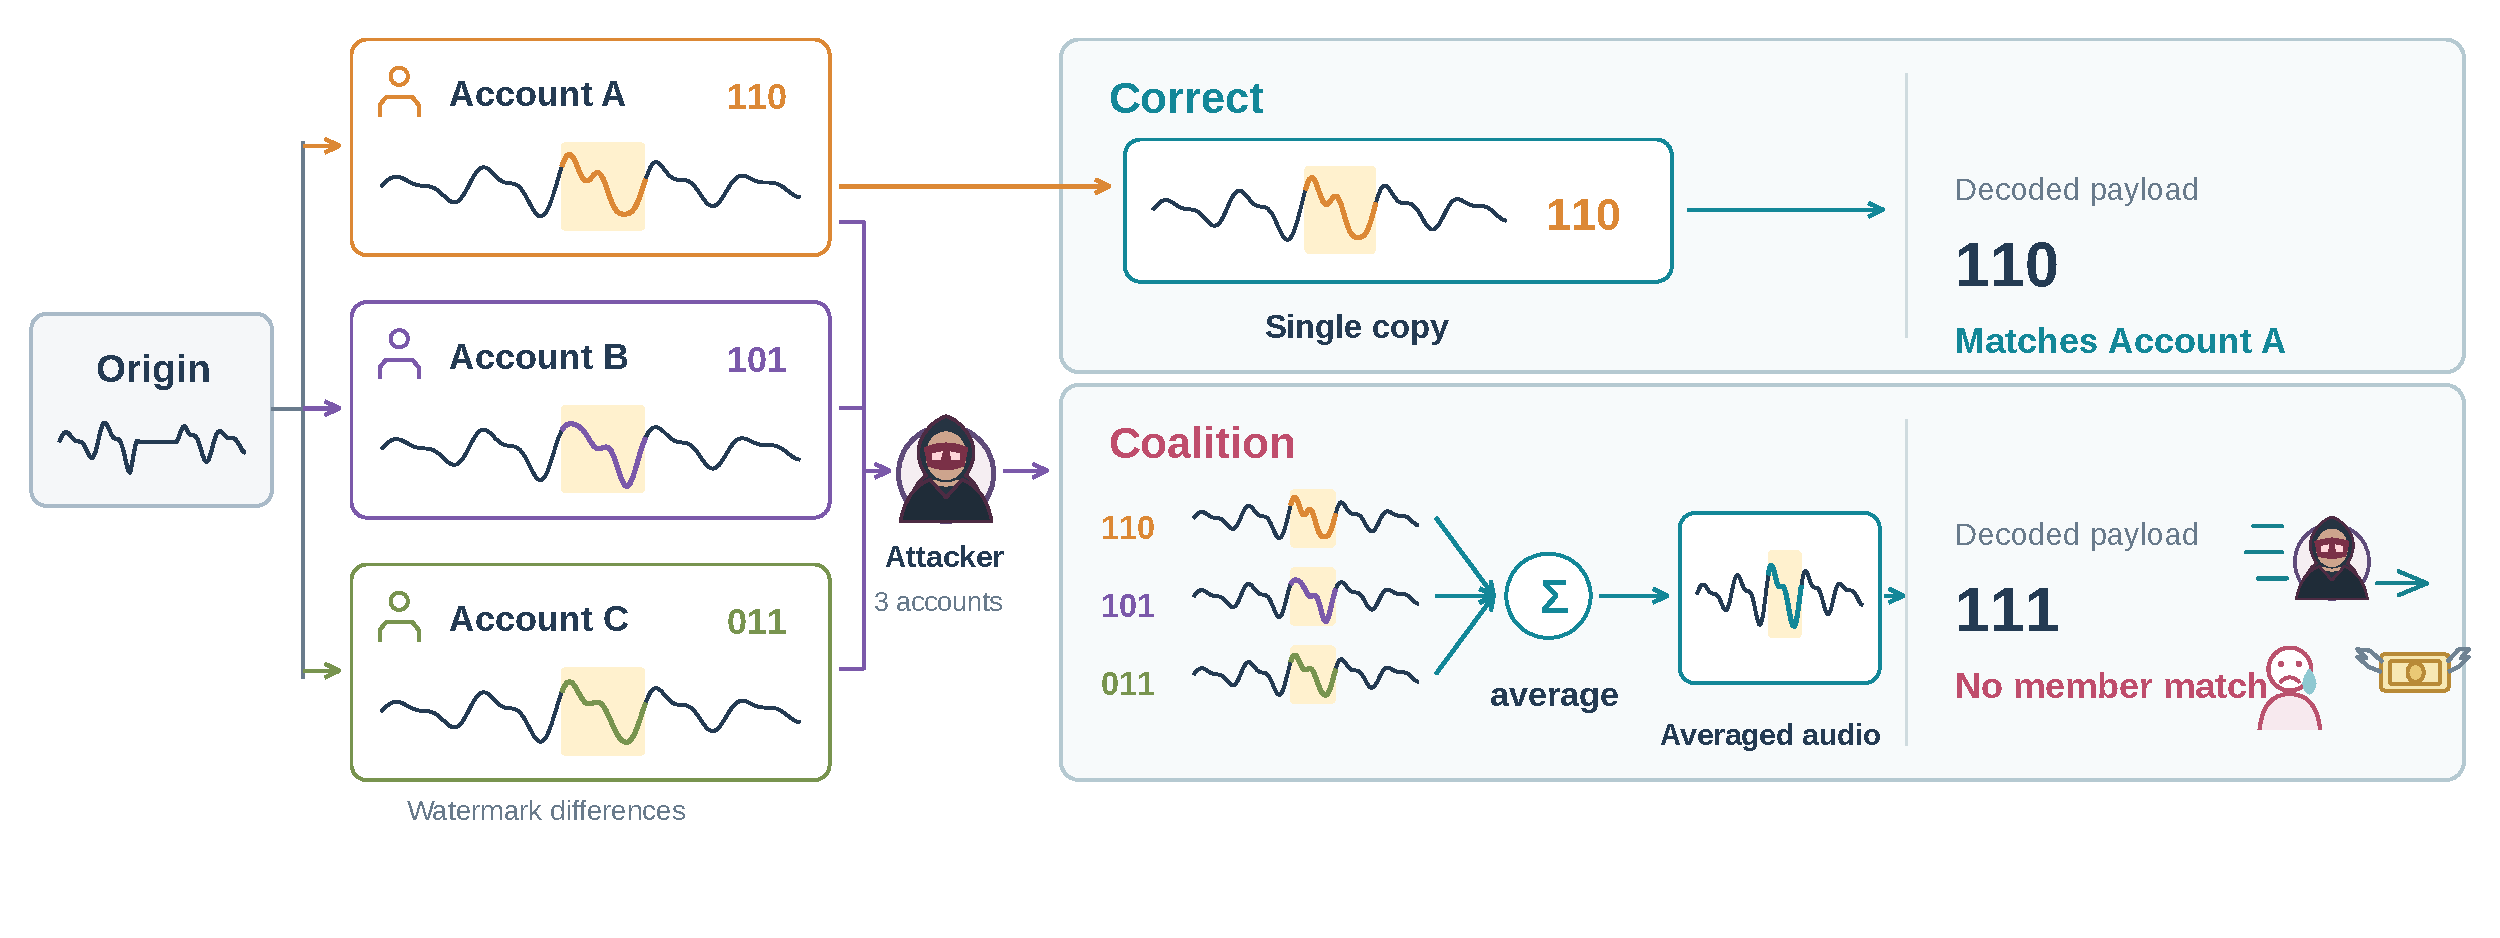
\includegraphics[width=0.88\textwidth,trim=11bp 52bp 13bp 15bp,clip]{fig1.pdf}
  \caption{A single copy traces its recipient. A coalition average can preserve the audio yet escape tracing.}
  \label{fig:scenario}
\end{figure*}

\begin{abstract}
Personalized audio watermarks trace a leaked copy to its recipient by decoding a recipient-specific payload. Existing evaluations typically transform one marked copy, leaving unanswered whether a decoder can still identify a coalition member after several valid copies are combined. We evaluate sample-wise averaging on five neural audio watermark systems using 300 ten-second utterances at coalition sizes 2, 3, 5, and 8. Every input copy decodes correctly before mixing. With only two copies, 86.3--99.3\% of mixtures yield payloads that match no coalition member. Mean PESQ remains 4.20--4.60 and mean STOI remains 0.983--0.999. The watermark is often preserved rather than erased: with eight copies, every non-tied TimbreWM bit follows the coalition majority, yet 92.0\% of complete payloads identify no member. Payload-only weighting produces a mean of 4.36--9.23 exact matches among ten selected nonmembers in three systems; the other two reach at most 0.13. Message recovery and recipient tracing are therefore distinct security objectives. Personalized watermark evaluations should test whether the complete decoded payload still identifies a coalition member after multiple valid copies are combined.
\end{abstract}

\begin{keywords}
audio watermarking, digital fingerprinting, recipient tracing, collusion, waveform averaging
\end{keywords}

\section{Introduction}

Personalized audio watermarking assigns a recipient-specific payload to each distributed copy. When a copy is leaked, the decoder recovers its payload and a registry identifies the recipient. Recipient tracing succeeds only if the complete decoded payload remains assigned to that recipient; watermark detection or partial bit recovery is not enough.

Coalition members can hold differently watermarked copies of the same recording. The speech waveform is shared, whereas the watermark residual depends on the assigned payload. A sample-wise average therefore preserves the common audio while combining the residuals, as illustrated in Fig.~\ref{fig:scenario}. The operation requires no clean recording, model access, payload knowledge, or added perturbation. Averaging directly tests whether a decoder trained on one payload per copy can still identify a coalition member when several valid payloads are present.

Neural audio watermark benchmarks mainly apply compression, noise, resampling, filtering, reconstruction, or replay to one marked copy and then report detection or message accuracy \cite{liu2024audiomarkbench,wang2024draw,li2024ideaw}. Classical fingerprinting instead treats collusion as a code-design and accusation problem \cite{cox1997spread,trappe2003anticollusion,boneh1998fingerprinting,tardos2003fingerprint,celik2004prewarping,tirkel2011audio}. Contemporary neural systems expose native payloads that applications can map to registry identities, but single-copy robustness does not establish that this mapping survives valid-copy averaging. The missing security test is recipient-level: after mixing copies that each decode correctly, does the complete output payload still identify a coalition member?

We answer that question across AudioSeal, WavMark, TimbreWM, VoiceMark, and WMCodec using their released payload spaces and native decoders \cite{sanroman2024audioseal,chen2023wavmark,liu2024timbre,li2025voicemark,zhou2024wmcodec}. At $K=2$, 86.3--99.3\% of averaged outputs escape tracing while speech quality remains high. Coalition-bit support and controlled one-bit mixtures show how decoder outputs can remain tied to the inputs without preserving any coalition member's complete payload. Weighted averaging then reaches selected nonmember payloads in three systems, showing that tracing escape can extend to targeted payload tampering in those systems. The results separate message recovery from recipient tracing and motivate coalition-aware evaluation.

\section{Threat Model and Evaluation}
\label{sec:evaluation}

The evaluation distinguishes the decoded message from the person being traced. A \emph{recipient} receives one personalized copy, a \emph{coalition member} contributes that copy to an average, and the \emph{payload} is the complete embedded bit string. A mixture \emph{escapes tracing} when its decoded payload matches none of the coalition members' assigned payloads. We report \emph{tracing failure} (TF) as the percentage of trials that escape. TF is therefore an outcome rate, not an attack method. Detection or high bit accuracy does not count as successful tracing unless the complete payload identifies a member.

Let $x$ be the shared speech waveform, $m_i$ the payload assigned to recipient $i$, and $w(x,m_i)$ the watermark residual. Recipient $i$ receives $y_i=x+w(x,m_i)$. For a coalition $\mathcal C$ of $K$ recipients, uniform averaging gives
\begin{equation}
  \bar y_K=\frac{1}{K}\sum_{i\in\mathcal C}y_i
  =x+\frac{1}{K}\sum_{i\in\mathcal C}w(x,m_i).
  \label{eq:mean}
\end{equation}
The shared waveform remains in Eq.~\eqref{eq:mean}; only the payload-dependent residuals are combined. This is the complete adversary requirement for the main experiment: aligned marked copies of the same recording.

Table~\ref{tab:systems} separates the systems by how their native decoder recovers a payload. AudioSeal, WavMark, and TimbreWM recover payload bits directly, so we call them bit-based. VoiceMark and WMCodec recover latent codes that map to payload bits, so we call them latent-based. We use each released decoder's native output rather than impose a common threshold.

\begin{table}[H]
\centering
\caption{Native payload decoders of the evaluated systems.}
\label{tab:systems}
\setlength{\tabcolsep}{4.2pt}
\begin{tabular}{lrl}
\toprule
System & Bits & Decoder \\
\midrule
AudioSeal \cite{sanroman2024audioseal} & 16 & Bit-based \\
WavMark \cite{chen2023wavmark} & 16 & Bit-based \\
TimbreWM \cite{liu2024timbre} & 10 & Bit-based \\
VoiceMark \cite{li2025voicemark} & 16 & Latent-based \\
WMCodec \cite{zhou2024wmcodec} & 16 & Latent-based \\
\bottomrule
\end{tabular}
\end{table}

% Register the double-column result table while TeX is still building page 2.
% The first explanatory reference remains above the bottom float in reading order.
\begin{table*}[!b]
\centering
\caption{TF and speech quality after uniform averaging (300 valid-input coalitions per cell).}
\label{tab:risk}
\setlength{\tabcolsep}{3.7pt}
\renewcommand{\arraystretch}{0.94}
\begin{tabular}{l*{12}{r}}
\toprule
& \multicolumn{3}{c}{$K=2$}
& \multicolumn{3}{c}{$K=3$}
& \multicolumn{3}{c}{$K=5$}
& \multicolumn{3}{c}{$K=8$} \\
\cmidrule(lr){2-4}\cmidrule(lr){5-7}\cmidrule(lr){8-10}\cmidrule(lr){11-13}
System
& TF (\%) & PESQ & STOI
& TF (\%) & PESQ & STOI
& TF (\%) & PESQ & STOI
& TF (\%) & PESQ & STOI \\
\midrule
AudioSeal
& 99.0 & 4.60 & 0.999
& 97.3 & 4.59 & 0.999
& 98.3 & 4.59 & 0.999
& 100.0 & 4.58 & 0.999 \\
WavMark
& 96.7 & 4.57 & 0.999
& 97.7 & 4.56 & 0.999
& 98.0 & 4.54 & 0.998
& 99.3 & 4.52 & 0.998 \\
TimbreWM
& 86.3 & 4.56 & 0.998
& 84.7 & 4.56 & 0.997
& 90.7 & 4.55 & 0.997
& 92.0 & 4.53 & 0.996 \\
VoiceMark
& 93.7 & 4.20 & 0.983
& 99.0 & 4.17 & 0.978
& 99.3 & 4.11 & 0.974
& 98.7 & 4.05 & 0.971 \\
WMCodec
& 99.3 & 4.37 & 0.989
& 99.3 & 4.32 & 0.986
& 100.0 & 4.26 & 0.984
& 99.7 & 4.24 & 0.983 \\
\midrule
\multicolumn{13}{l}{\textit{Ideal recombination}} \\
16-bit payload
& 97.9 & \multicolumn{2}{c}{--}
& 99.5 & \multicolumn{2}{c}{--}
& 99.9 & \multicolumn{2}{c}{--}
& 99.9 & \multicolumn{2}{c}{--} \\
10-bit payload
& 89.1 & \multicolumn{2}{c}{--}
& 94.3 & \multicolumn{2}{c}{--}
& 96.8 & \multicolumn{2}{c}{--}
& 97.4 & \multicolumn{2}{c}{--} \\
\bottomrule
\end{tabular}

\end{table*}

Every experiment unit uses 300 ten-second utterances from 100 speakers, with three different utterances per speaker. The set contains 50 Mandarin speakers from AISHELL-3 and 50 English speakers from LibriSpeech \cite{shi2021aishell3,panayotov2015librispeech}. We test $K\in\{2,3,5,8\}$. For each utterance, system, and $K$, we sample distinct payloads and embed one personalized copy per payload. We include a coalition only when every input copy decodes exactly to its assigned payload. A pre-existing single-copy error therefore cannot create a false tracing escape.

Embedding, averaging, and decoding use each system's native sampling rate: 16~kHz for AudioSeal, WavMark, and VoiceMark; 22.05~kHz for TimbreWM; and 24~kHz for WMCodec. Payload sampling and registry lookup use the same bit order. A fixed manifest and deterministic seeds record the speaker, utterance, payloads, decoded output, mixture weights, and quality scores for every trial.

PESQ and STOI measure how much averaging changes the distributed audio \cite{rix2001pesq,taal2011stoi}. The reference is the first valid personalized copy in the coalition and the test signal is the average. The scores therefore measure the additional change caused by combining copies, not the watermark's distortion relative to clean speech.

We use \emph{ideal recombination} to show the TF expected when coalition bits survive but no member's complete payload is preserved. At each bit, it copies the value of one uniformly selected coalition member. If six of eight members carry 1, the ideal output is 1 with probability $6/8$. We then assemble the bits and apply the same exact-match test as for the audio systems.

\section{Recipient Tracing Under Collusion}
\label{sec:main_results}

\subsection{Uniform Averaging Causes Tracing Escape}

The main failure appears at the smallest coalition size. Table~\ref{tab:risk} shows 86.3--99.3\% TF at $K=2$ across the five systems. The corresponding mean PESQ is 4.20--4.60 and STOI is 0.983--0.999. Thus, the output usually escapes tracing while the shared speech remains close to a valid personalized input.

Increasing the coalition from two to eight does not create the vulnerability; TF remains between 84.7\% and 100.0\%. The audio remains high quality over the same range: the lowest reported means are 4.05 PESQ and 0.971 STOI, both for VoiceMark at $K=8$. The mixtures therefore escape tracing without a collapse in speech quality.

Ideal recombination already produces 97.9--99.9\% TF for 16-bit payloads and 89.1--97.4\% for 10-bit payloads. The five systems remain close to those ranges. High TF is therefore consistent with coalition bits surviving but being assembled into a payload that belongs to no member. Figure~\ref{fig:composition} tests that explanation directly.

\subsection{Bit Recombination Explains the Escape}
\label{sec:composition}

TF alone cannot show whether averaging erases the watermark or recombines coalition bits. Figure~\ref{fig:composition} answers this at $K=8$. For each bit, the horizontal axis counts how many of the eight members carry 1, and the vertical axis reports how often the decoder outputs 1. Counts 0 and 8 are unanimous inputs, 4 is a tie, and the gray $c/8$ line shows ideal bit mixing.

\begin{figure}[H]
  \centering
  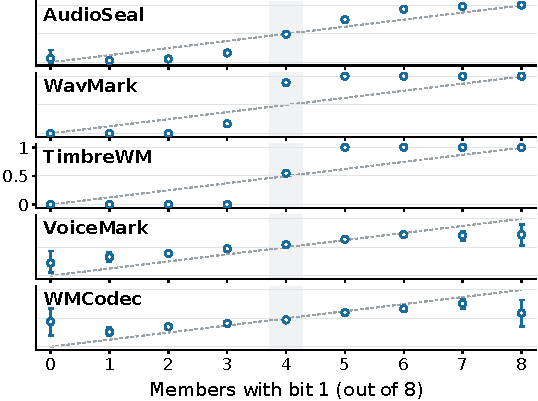
\includegraphics[width=\columnwidth]{fig2.pdf}
  \caption{Coalition support (horizontal) and decoded-one rate (vertical) at $K=8$. The dashed line is Ideal; whiskers show 95\% speaker-bootstrap intervals.}
  \label{fig:composition}
\end{figure}

The figure separates two response patterns. AudioSeal, WavMark, and TimbreWM follow coalition support in 84.9--100.0\% of non-tied bits; AudioSeal changes gradually, whereas WavMark and TimbreWM switch sharply around the tie. VoiceMark and WMCodec follow the input bits less consistently, even when every coalition member supplies the same value.

Bit agreement does not restore recipient tracing. A three-bit example makes the distinction explicit: the bit-wise majority of 110, 101, and 011 is 111, although no coalition member carries 111. Table~\ref{tab:k8} applies that logic to the full payload. ``Majority bits'' is the fraction of non-tied bits that follow the coalition majority. ``All majority bits'' is the fraction of trials that follow it at every non-tied bit.

\begin{table}[H]
\centering
\caption{How decoded bits follow coalition bit values at $K=8$.}
\label{tab:k8}
\setlength{\tabcolsep}{2.2pt}
\begin{tabular}{lrrr}
\toprule
System & \shortstack{Majority\\bits (\%)} & \shortstack{Unanimous\\bits (\%)} & \shortstack{All majority\\bits (\%)} \\
\midrule
AudioSeal & 84.9 & 96.7 & 20.7 \\
WavMark & 95.0 & 100.0 & 54.3 \\
TimbreWM & 100.0 & 100.0 & 100.0 \\
VoiceMark & 61.9 & 74.3 & 0.7 \\
WMCodec & 62.5 & 59.7 & 1.0 \\
\bottomrule
\end{tabular}

\end{table}

TimbreWM supplies the clearest contradiction between bit recovery and tracing: every non-tied bit follows the majority and every unanimous bit is retained, yet 92.0\% of complete payloads match no coalition member. AudioSeal and WavMark show the same recombination effect less perfectly. Coalition-supported bits can therefore form a complete payload assigned to no coalition member. VoiceMark and WMCodec follow coalition bits less consistently, but their complete payloads still escape tracing.

\subsection{Mixing Can Change Bits Shared by Both Inputs}
\label{sec:one_bit}

Bit recombination does not explain why VoiceMark can change a bit shared by all inputs. We isolate that behavior with two valid copies that differ at exactly one bit. AudioSeal represents bit-based decoding and VoiceMark represents latent-based decoding. For 300 source-correct pairs per system, we vary the weight on the second copy from 0 to 1. Any decoded payload other than the two endpoints must contain a change at a bit where both inputs agree.

\begin{figure}[!t]
  \centering
  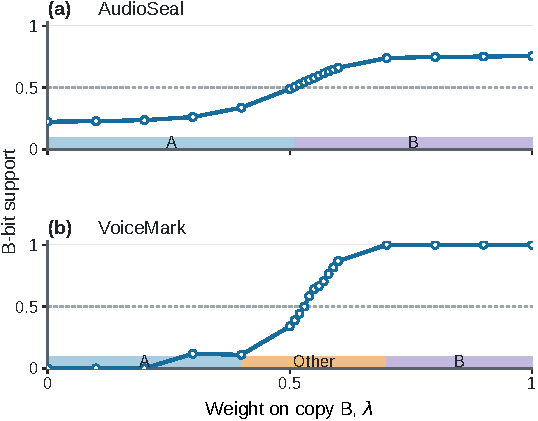
\includegraphics[width=\columnwidth]{fig3.pdf}
  \caption{Decoder support for B's differing bit versus B's mixture weight. The strip shows the decoded payload: A, B, or Other.}
  \label{fig:paths}
\end{figure}

AudioSeal moves directly between the two valid payloads in 299 of 300 paths (99.7\%). VoiceMark visits another payload in 187 of 300 paths (62.3\%), so at least one originally shared bit also changes. The contrast shows that a latent-based decoder can change a bit shared by both inputs.

\section{Targeted Payload Tampering}
\label{sec:tampering}

Tracing escape and targeted payload tampering are different claims. An escape may point anywhere outside the coalition. Targeted payload tampering succeeds only when the decoded complete payload equals a nonmember chosen before the waveform is decoded. We test exact full-payload matches among targets selected from each system's native registry; a partial bit match or merely approaching a target does not count.

Two payload-only rules choose both targets and mixture weights. Payload matching (PM) is inspired by the bitwise message objectives used in learned watermark decoders \cite{tancik2020stegastamp,luo2020distortion}: it selects the ten nonmembers closest to the coalition's weighted payloads and caps each waveform weight at 0.5. The margin rule (MRC) instead favors targets whose least-supported bit can be moved farther across its decision boundary. It uses smooth-min temperature 8, entropy weight 0.05, and requires an effective coalition size $1/\sum_i a_i^2\geq0.6K$. Both methods use nonnegative weights that sum to one and do not query the audio decoder while choosing them.

Each method ranks the full registry after removing coalition members, selects ten nonmembers, and creates one weighted mixture per target. We count exact decoded matches on a direct 0--10 scale: reaching four targets contributes 4, not 1. The ten hits are summed within each trial and then averaged over 300 trials. AudioSeal, WavMark, VoiceMark, and WMCodec use the same coalitions; TimbreWM uses its own valid-input coalitions because its payload has 10 rather than 16 bits. Table~\ref{tab:targets} compares the complete PM and MRC procedures, including their different target choices.

\begin{table}[!t]
\centering
\caption{Mean exact matches among ten selected nonmember targets (0--10).}
\label{tab:targets}
\setlength{\tabcolsep}{3.1pt}
\begin{tabular}{lrrrr}
\toprule
& \multicolumn{2}{c}{PM} & \multicolumn{2}{c}{MRC} \\
\cmidrule(lr){2-3}\cmidrule(lr){4-5}
System & $K=5$ & $K=8$ & $K=5$ & $K=8$ \\
\midrule
AudioSeal & 2.39 & 3.57 & 4.19 & 4.36 \\
WavMark   & 2.59 & 3.55 & 5.14 & 5.44 \\
TimbreWM  & 3.93 & 6.07 & 7.84 & 9.23 \\
VoiceMark & 0.17 & 0.20 & 0.11 & 0.06 \\
WMCodec   & 0.16 & 0.18 & 0.10 & 0.13 \\
\bottomrule
\end{tabular}

\end{table}

At $K=8$, MRC reaches 4.36--9.23 of ten selected targets for AudioSeal, WavMark, and TimbreWM, versus at most 0.13 for VoiceMark and WMCodec. The $K=5$ results repeat this split, and speaker-bootstrap intervals do not overlap. PM gives the same grouping but fewer hits. Quality remains high (mean PESQ 3.92--4.58; STOI 0.968--0.999). Selected-target control therefore occurs in three systems, not for arbitrary recipients across all five.

\section{Confidence of Tampered Payloads}
\label{sec:confidence}

Coalition-supported bits can recombine, and some decoders change additional bits during mixing. Neither observation shows how strongly the decoder accepts the least certain bit in its final payload. Figure~\ref{fig:confidence} tests whether a successful MRC target merely crosses a decision boundary or receives stronger support. In the three readily targeted systems, MRC increases that minimum support but leaves a visible gap to valid copies.

For each decoded payload, we retain the lowest confidence among its bits. A decoded 1 uses the probability or vote share for 1; a decoded 0 uses the support for 0. This is bit confidence, not watermark-detection confidence. AudioSeal and TimbreWM provide bit probabilities, VoiceMark and WMCodec outputs are converted to bit probabilities, and WavMark uses the share of valid windows voting for the decoded value. Because these outputs are not calibrated across systems, only comparisons within the same system are meaningful.

\begin{figure}[H]
  \centering
  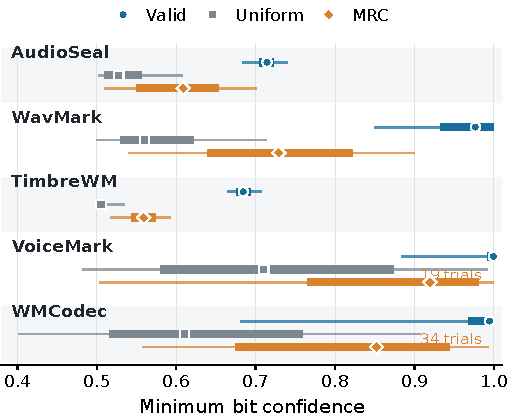
\includegraphics[width=\columnwidth]{fig4.pdf}
  \caption{Minimum bit confidence at $K=8$. Points show medians; thick and thin lines show the middle 50\% and 90\% of trials.}
  \label{fig:confidence}
\end{figure}

Figure~\ref{fig:confidence} compares Valid, Uniform, and MRC in that top-to-bottom order. MRC shows the highest-ranked exact target match in each trial, so the row measures confidence conditional on successful tampering; Table~\ref{tab:targets} reports how often those matches occur. The first three systems succeed in nearly every trial. VoiceMark and WMCodec provide only 19 and 34 matches, as marked in the figure.

The three readily targeted systems share one pattern: the median minimum confidence is 0.05--0.17 higher for MRC than for Uniform, but remains below Valid. Their middle 50\% ranges also remain separate from Valid. Successful tampering therefore moves the least certain bit farther into the decoded target without making the output fully resemble a valid copy. The sparse VoiceMark and WMCodec matches cannot describe their usual behavior. This comparison is descriptive, because MRC already favors targets with stronger payload-side support.

\section{Discussion}
\label{sec:discussion}

Single-copy message recovery is insufficient evidence for recipient tracing. Every tested coalition begins with input copies that decode correctly, yet the averaged payload usually identifies no coalition member. Evaluations of personalized watermarks should therefore add a multi-copy test with valid inputs and compare the complete decoded payload directly with the coalition members' assignments. Detection rate and bit accuracy answer different questions and cannot stand in for that exact match.

The experiments also expose two decoder response patterns. AudioSeal, WavMark, and TimbreWM track coalition bit support and allow frequent exact hits among selected nearby targets. VoiceMark and WMCodec show weaker bit agreement; the controlled VoiceMark paths confirm that a bit shared by both inputs can also change. Neither pattern preserves tracing: the first permits recombination and control, while the second produces mostly uncontrolled nonmember payloads. Reporting only TF would hide that difference.

Confidence-based rejection is a design direction, not a conclusion already validated by Fig.~\ref{fig:confidence}. A tracer could calibrate its lowest bit confidence on separate valid copies and decline a recipient assignment when a new output falls outside that range. No universal threshold follows from our data because confidence is not calibrated across systems. A confidence rule will also be insufficient when successful mixtures overlap the valid-copy range; payload redundancy, collusion-aware recipient codes, or checks across decoding windows may then be needed. The central requirement is that a decoder may return ``no reliable recipient'' instead of forcing every detected watermark to a registry entry.

\section{Conclusion}
\label{sec:conclusion}

Waveform averaging can preserve audio quality and watermark evidence while breaking recipient tracing. Across five systems, valid-copy averaging produced mostly nonmember payloads; three systems also admitted exact matches to selected nonmembers under payload-only weighting. These results separate message recovery from recipient assignment. Personalized watermark evaluation should therefore include multi-copy tests and verify whether the complete decoded payload still identifies a coalition member.

\bibliographystyle{IEEEbib}
\bibliography{references}
\end{document}
